% Created 2022-09-15 Thu 18:20
% Intended LaTeX compiler: pdflatex
\documentclass[presentation]{beamer}
\usepackage[utf8]{inputenc}
\usepackage[T1]{fontenc}
\usepackage{graphicx}
\usepackage{longtable}
\usepackage{wrapfig}
\usepackage{rotating}
\usepackage[normalem]{ulem}
\usepackage{amsmath}
\usepackage{amssymb}
\usepackage{capt-of}
\usepackage{hyperref}
\setbeamertemplate{navigation symbols}{}
\setbeamerfont{caption}{size=\scriptsize}
\AtBeginSection[]{\begin{frame}\frametitle{Table of Contents}\tableofcontents[currentsection]\end{frame}}
\usetheme{default}
\setcounter{secnumdepth}{2}
\author{Paul Etheimer}
\date{\today}
\title{REMC for Protein Folding}
\hypersetup{
 pdfauthor={Paul Etheimer},
 pdftitle={REMC for Protein Folding},
 pdfkeywords={},
 pdfsubject={},
 pdfcreator={Emacs 28.1 (Org mode 9.6)}, 
 pdflang={English}}
\usepackage{biblatex}

\begin{document}

\maketitle
\begin{frame}{Outline}
\tableofcontents
\end{frame}

\section{Introduction}
\label{sec:org47d9eab}
\begin{frame}[label={sec:org92d9e4b}]{Monte Carlo Algorithms}
\begin{definition}[MC algorithm]
A Monte Carlo algorithm is a problem solving procedures that uses randomness to approach a solution too complex to solve deterministically.
\end{definition}
\end{frame}
\begin{frame}[label={sec:org6927040}]{The HP protein folding model}
\begin{definition}[HP model]
The Hydrophobic-Polar protein folding model is a highly simplified model of protein folding in space, that relies on the dominance of the \emph{hydrophobic effect} on soluble protein folding. It sorts amino acid in two categories, hydrophobic or polar.
\end{definition}
\end{frame}
\begin{frame}[label={sec:orgddbb716}]{The Replica Exchange Monte Carlo}
\begin{definition}[REMC]
The Replica Exchange Monte Carlo (or parallel tempering), is a type of MC algorithm. It runs parallelly multiple MC models, at different temperatures, and exchanges them based on their energy.
\end{definition}
\end{frame}
\begin{frame}[label={sec:org86d4f4a}]{The VSHD neighbourhood}
\begin{columns}
\begin{column}{.6\columnwidth}
\begin{figure}[htbp]
\centering
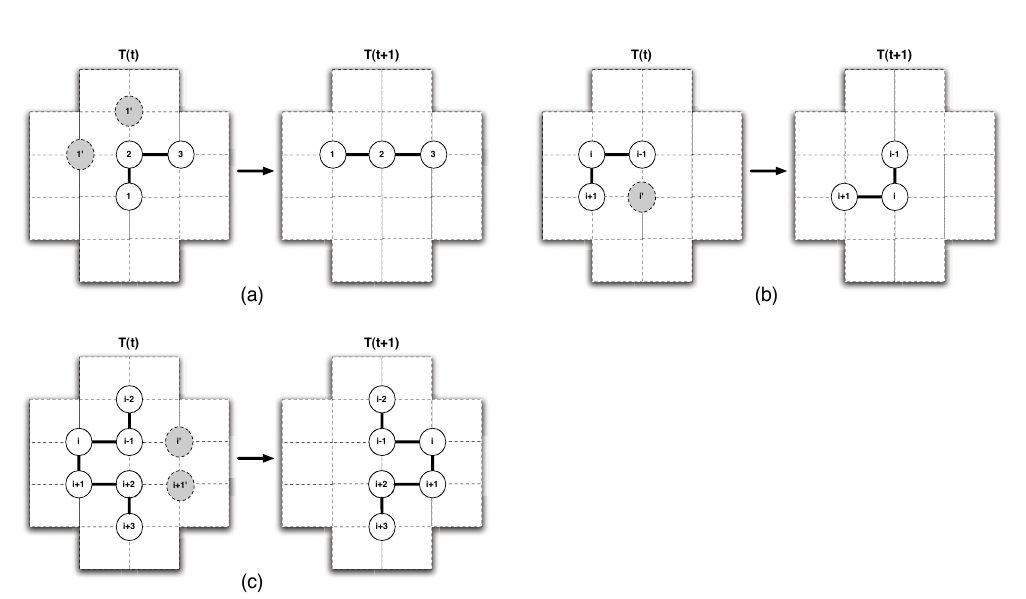
\includegraphics[width=200px]{./vshd.png}
\caption{\label{fig:moves}The 3 moves implemented : (a) end move (b) corner move (c) crankshaft move (figure from the article)}
\end{figure}
\end{column}

\begin{column}{.3\columnwidth}
\begin{definition}[VSHD]
A \emph{neighbourhood} of exploration, consisting of three moves a conformation can perform:
\begin{itemize}
\item an \emph{end move} (only for end residues)
\pause
\item \emph{corner move}
\pause
\item \emph{crankshaft move}
\end{itemize}
\end{definition}
\end{column}
\end{columns}
\end{frame}
\section{Implementation}
\label{sec:org11e5732}
\begin{frame}[label={sec:org7d889c4},fragile]{Object-oriented programming}
 \begin{itemize}
\item Python 3.10 with numpy 1.22
\pause
\item 3 classes:
\begin{itemize}
\item AminoAcid - A basic amino acid, attributes: \texttt{position, hp\_type, index}
\item Conformation - The main class, attributes: \texttt{lattice, amino\_list, sequence, energy, line}
\item Move - a class for movement, attributes: \texttt{move\_type, conf, number, new\_position, old\_position}
\end{itemize}
\end{itemize}
\end{frame}
\begin{frame}[label={sec:orgdc742af}]{The class relations}
\begin{figure}[htbp]
\centering
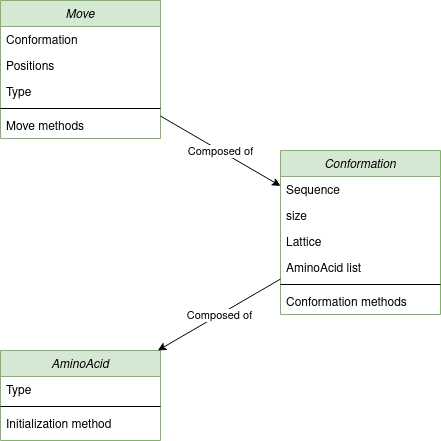
\includegraphics[width=200px]{./classes.png}
\caption{\label{fig:cls}The 3 classes implemented and their relationships}
\end{figure}
\end{frame}
\begin{frame}[label={sec:org629fdc9},fragile]{Two functions and a main}
 \begin{itemize}
\item \texttt{mc\_search}: Takes a conformation, drives its evolution step by step (internal loop)
\pause
\item \texttt{remc}: Orchestrates all the replicas, stopping either at a target energy or at a specified maximum number of steps
\pause
\item \texttt{main.py}: Parses the arguments with \texttt{argparse}, creates the conformation and runs the optimization
\end{itemize}
\end{frame}
\begin{frame}[label={sec:org64becc6}]{Around the program}
\begin{itemize}
\item Used podman - but limitation to files entry in a CLI
\item Used conda for file handling
\end{itemize}
\end{frame}

\section{Results}
\label{sec:org7f585e6}
\begin{frame}[label={sec:orgafcf54e}]{Middling at best}
\begin{itemize}
\item Slow algorithm: two minutes for 110 residues with 5000 total steps (with random walk initialization)
\pause
\item Buggy crankshaft moves
\pause
\item Not much movement without \emph{pull moves}, especially with a line start position
\end{itemize}
\end{frame}
\section{Discussion - Post mortem}
\label{sec:org1878883}
\begin{frame}[label={sec:org056020b},fragile]{Bad decisions}
 \begin{itemize}
\item The exaggerated OOP (\texttt{Move}) and deepcopy usage
\end{itemize}
\pause
\begin{itemize}
\item No reproducible examples
\end{itemize}
\pause
\begin{itemize}
\item No non-random test environment
\end{itemize}
\end{frame}


\begin{frame}[label={sec:org4540021}]{Knowledge limits}
\begin{itemize}
\item Lack of knowledge about debugging in Python
\pause
\item Lack of knowledge about performance profiling in Python
\end{itemize}
\end{frame}




\begin{frame}[label={sec:orgabe209f}]{Tool limits}
\begin{itemize}
\item Manipulating heavy lattices is unwieldly in Python
\end{itemize}
\pause
\begin{itemize}
\item Python is a slow language, especially with low-level programs such as this
\end{itemize}
\end{frame}

\begin{frame}[label={sec:orge851777}]{Paper limits}
\begin{columns}
\begin{column}{.3\columnwidth}
\begin{itemize}
\item At least a mistake : a wrong comparison sign cost a lot of time
\item The omission of the mention of the usage of the Boltzmann constant is also surprising
\end{itemize}
\end{column}
\begin{column}{.6\columnwidth}
\begin{figure}[htbp]
\centering
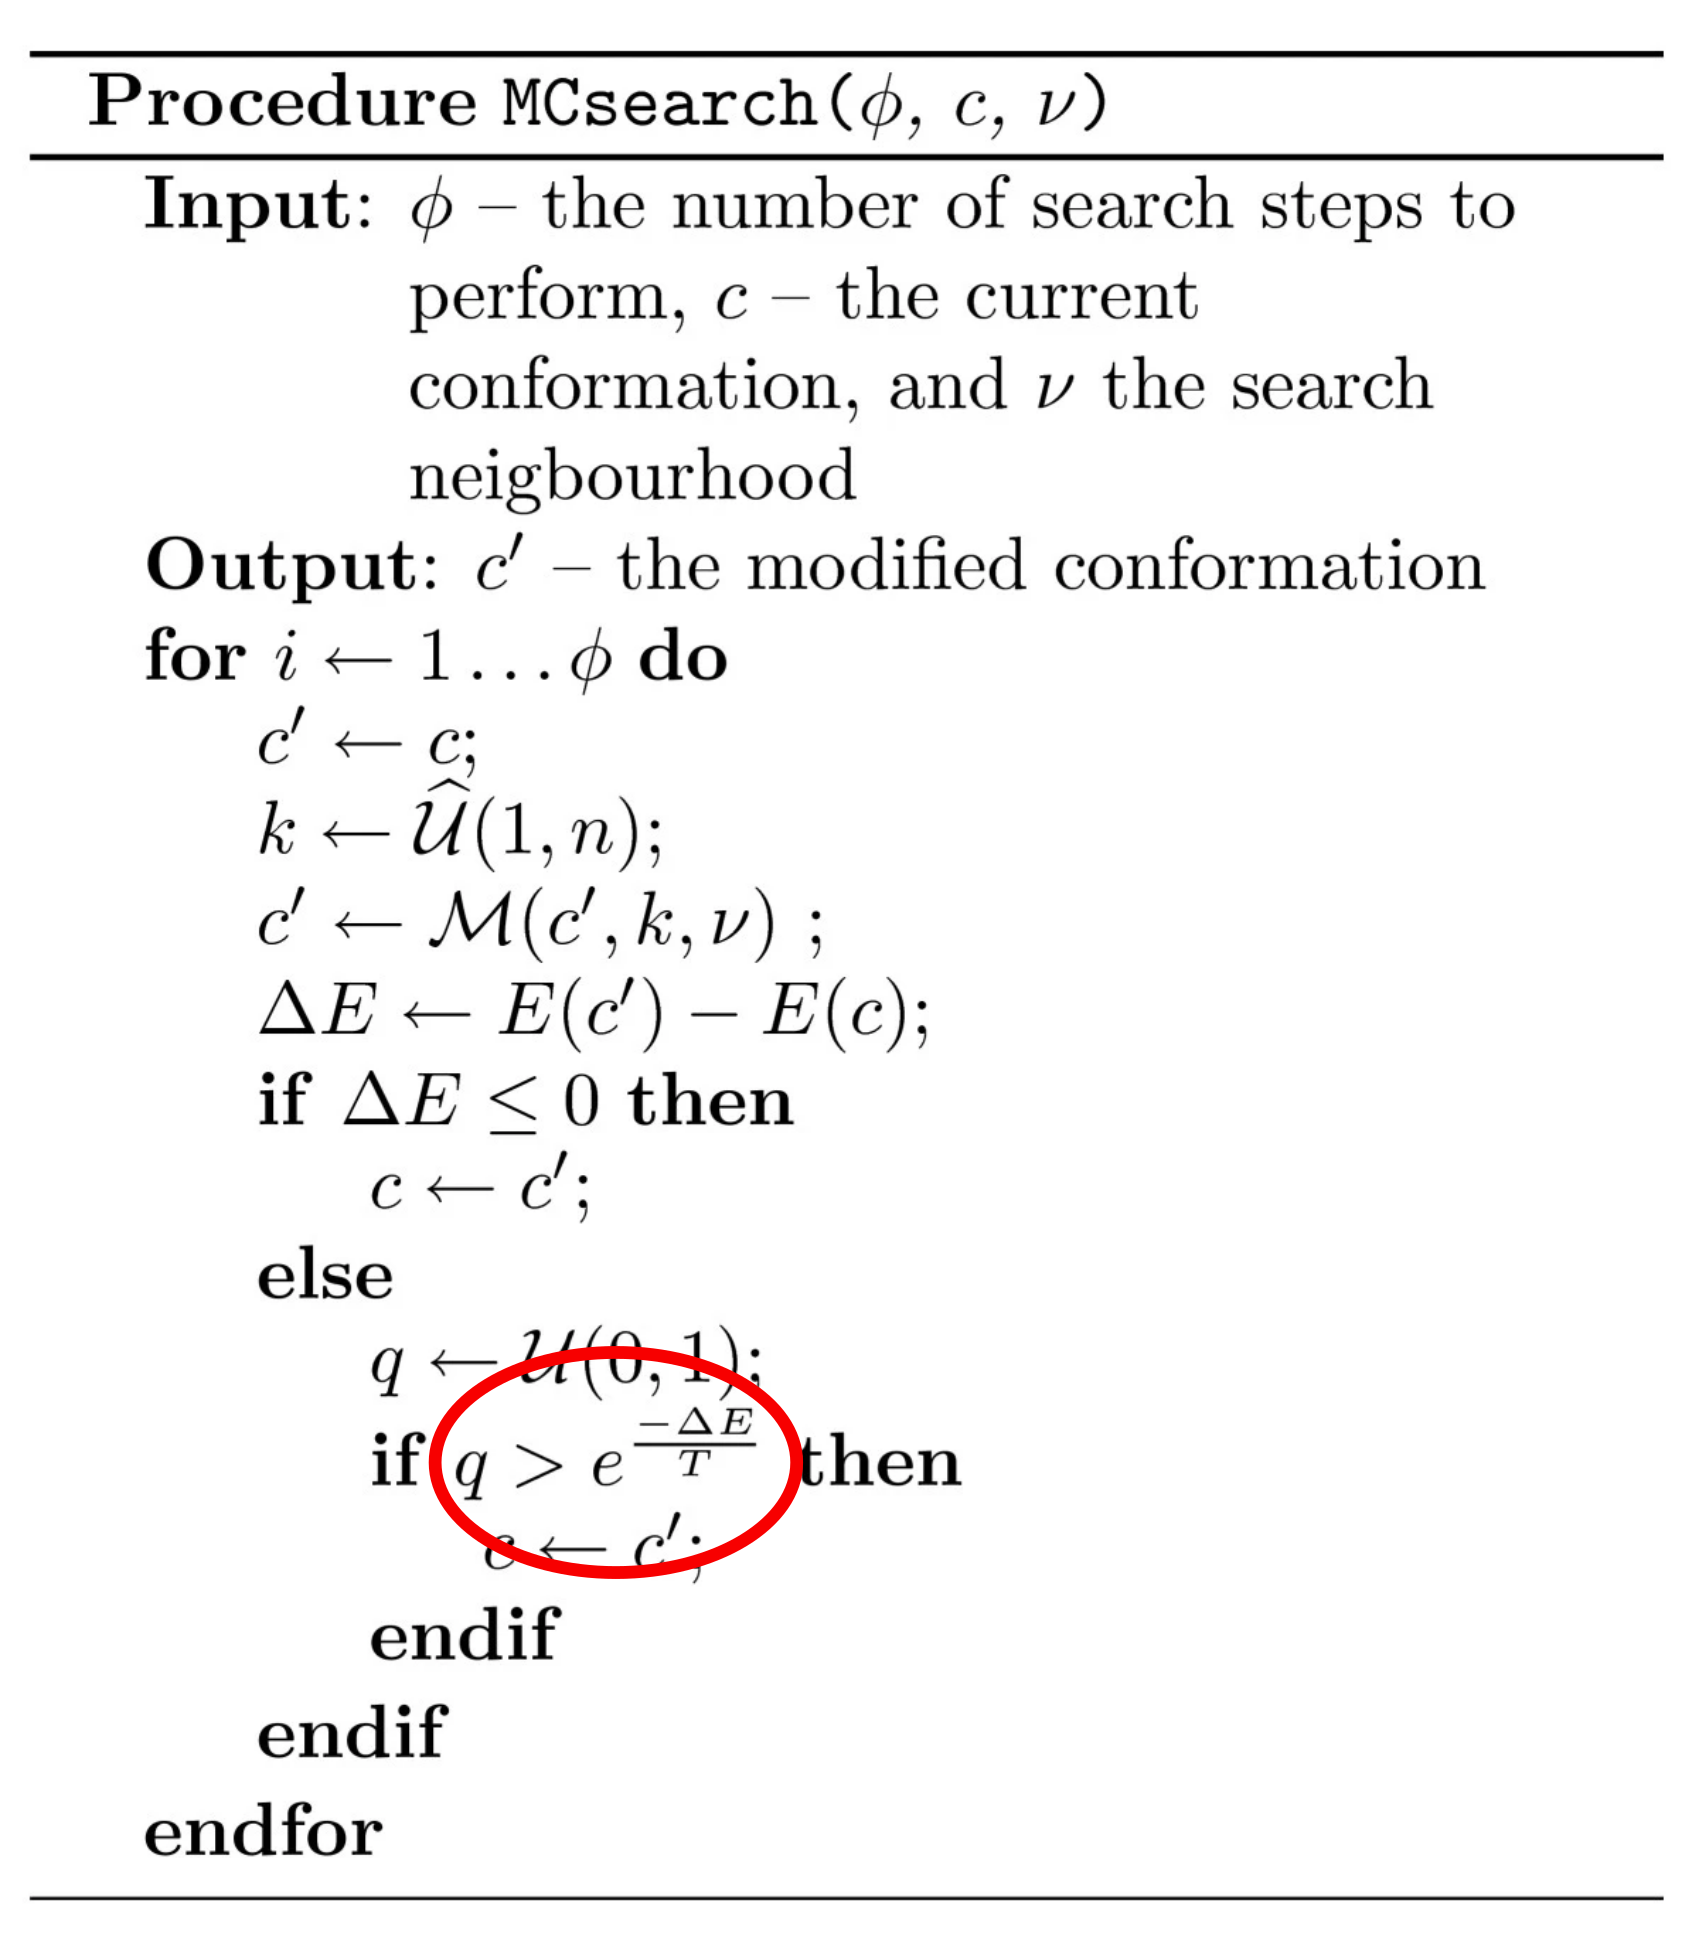
\includegraphics[width=170px]{./figure_red.png}
\caption{\label{fig:cls}The problematic \textbf{>} sign}
\end{figure}
\end{column}
\end{columns}
\end{frame}

\begin{frame}[label={sec:orgd12fa27}]{Thank you}
\huge{\center Questions?}
\end{frame}
\end{document}
